% =========================================================
% Artículo Científico - TPI Algoritmos Genéticos
% Algoritmos Genéticos aplicados al Scheduling de Alertas en un SOC
% Universidad Tecnológica Nacional - Facultad Regional Rosario
%
% Formato ajustado a "Formato para la presentación de Documentos"
% de la cátedra: Times New Roman, A4, márgenes 2.5cm, dos columnas
% con 1cm de separación, sin numeración de página.
%
% Compilar con XeLaTeX (usa fontspec para Times New Roman):
%   xelatex articulo.tex   (correr dos veces para resolver referencias)
% =========================================================
\documentclass[12pt,a4paper]{article}

\usepackage{fontspec}
\setmainfont{Times New Roman}

\usepackage[margin=2.5cm]{geometry}
\usepackage{amsmath}
\usepackage{graphicx}
\PassOptionsToPackage{hyphens}{url}
\usepackage{hyperref}

\setlength{\columnsep}{1cm}
\pagestyle{empty}
\tolerance=1200
\emergencystretch=3em
\hbadness=10000

\hypersetup{
  colorlinks=true,
  linkcolor=black,
  urlcolor=black,
  citecolor=black
}

\renewcommand{\refname}{Referencias}

% ---------------------------------------------------------
% Comandos de estilo según el formato de la cátedra
% ---------------------------------------------------------
\newcommand{\artTitle}[1]{{\fontsize{16}{19}\selectfont\bfseries #1\par}}
\newcommand{\artAuthors}[1]{{\fontsize{14}{17}\selectfont\bfseries #1\par}}
\newcommand{\artInstitution}[1]{{\fontsize{12}{15}\selectfont\bfseries\itshape #1\par}}
\newcommand{\artLabel}[1]{{\fontsize{10}{12}\selectfont\bfseries #1}}
\newcommand{\artSmall}{\fontsize{10}{12}\selectfont}

\newcommand{\artSection}[1]{%
  \par\vspace{0.7em}
  {\fontsize{12}{15}\selectfont\bfseries #1\par}
  \vspace{0.3em}
}

\newcounter{tabla}
\newcommand{\artTablaCaption}[1]{%
  \refstepcounter{tabla}%
  \par\noindent{\artSmall\itshape Tabla \thetabla. #1\par}\vspace{0.3em}
}

\newcounter{figuraart}
\newcommand{\artFiguraCaption}[1]{%
  \refstepcounter{figuraart}%
  \par\noindent{\artSmall\itshape Figura \thefiguraart. #1\par}\vspace{0.3em}
}

\begin{document}

% ---------------------------------------------------------
% Bloque de título a ancho completo (título, autores,
% institución, abstract, palabras clave)
% ---------------------------------------------------------
\twocolumn[
  \begin{center}
    \artTitle{Algoritmos Genéticos aplicados al Scheduling de Alertas\\en un Centro de Operaciones de Seguridad (SOC)}
    \vspace{0.6em}
    \artAuthors{Chacón, A.\ ; Gomez Manna, J.\ ; Tabini, A.\ ; Carloni, N. I.\ ; Mierez, J.}
    \vspace{0.2em}
    \artInstitution{Universidad Tecnológica Nacional, Facultad Regional Rosario}
  \end{center}
  \vspace{1em}

  \noindent\artLabel{Abstract}\ {\artSmall\itshape
  Los Centros de Operaciones de Seguridad (SOC) reciben un volumen de alertas que crece más rápido que la disponibilidad de analistas capacitados para atenderlas, lo que produce sobrecarga, fatiga de alertas y desbalance de carga cuando la asignación se realiza de forma manual o con reglas fijas. Este trabajo propone modelar la asignación de alertas a analistas como un problema de optimización combinatoria y resolverlo mediante un Algoritmo Genético Canónico, con selección de padres por ruleta, cruza de un punto y mutación por reasignación. Cada cromosoma codifica una asignación completa de alertas a analistas, y su aptitud se evalúa con una función de fitness que combina el tiempo total estimado de resolución con penalizaciones por espera, incumplimiento de SLA en alertas críticas, backlog y desbalance de carga. Se evaluó el modelo sobre 500 alertas derivadas de una muestra real del dataset público CICIDS2017. El algoritmo convergió hacia una asignación con un fitness de 5,9584$\times10^{-5}$, un tiempo total estimado de 2377 minutos y un desbalance de carga de 0,0873 entre los 10 analistas. Los resultados confirman que el modelo propuesto constituye una alternativa formal, medible y reproducible frente a las heurísticas manuales de asignación actualmente en uso en los SOC.
  \par}

  \vspace{0.6em}
  \noindent\artLabel{Palabras Clave}\ {\artSmall Algoritmos genéticos; scheduling; balanceo de carga; Centro de Operaciones de Seguridad; metaheurísticas; optimización combinatoria; selección genética; alert fatigue.\par}
  \vspace{1.2em}
]

% ---------------------------------------------------------
% Introducción
% ---------------------------------------------------------
\artSection{Introducción}

Un Centro de Operaciones de Seguridad (SOC) es el equipo y la infraestructura responsables de monitorear, detectar y responder a incidentes de ciberseguridad en una organización, a partir de las alertas centralizadas por plataformas de gestión de eventos e información de seguridad (SIEM). Cuando el volumen de alertas supera la capacidad de análisis manual se produce sobrecarga de alertas (\textit{alert overload}) (Jalalvand et al., 2025) \cite{ref1}, y cuando esa sobrecarga se sostiene en el tiempo degrada la calidad de las decisiones de triaje, fenómeno conocido como fatiga de alertas (\textit{alert fatigue}) (Tariq et al., 2025) \cite{ref2}. A esta escasez estructural se suma un problema de coordinación: las prácticas habituales de asignación --turnos fijos, reglas estáticas o asignación manual-- no consideran de forma simultánea la prioridad de cada alerta, el plazo comprometido (SLA), el tiempo estimado de resolución y la carga ya acumulada por cada analista, lo que produce desbalance de carga y riesgo de incumplimiento en alertas críticas.

Frente a este panorama, el presente trabajo formula la asignación de alertas como un problema de optimización combinatoria y propone resolverlo mediante un Algoritmo Genético Canónico. El objetivo general es diseñar, implementar y evaluar un modelo de este tipo que minimice de forma conjunta el tiempo total de resolución, el incumplimiento de los SLA en alertas críticas, el backlog y el desbalance de carga entre analistas de un SOC.

% ---------------------------------------------------------
% Elementos del trabajo y metodología
% ---------------------------------------------------------
\artSection{Elementos del trabajo y metodología}

El modelo representa el estado de un SOC compuesto por un conjunto fijo de analistas y un conjunto de alertas, cada una caracterizada por su prioridad, severidad, tiempo estimado de resolución y SLA asociado. Las 500 alertas evaluadas se derivaron de una muestra aleatoria de \textbf{CICIDS2017} \cite{ref6}, un dataset público de 225.745 flujos de red de una captura con ataque DDoS, etiquetados como \texttt{DDoS} o \texttt{BENIGN}. Como el dataset no incluye campos operativos de SOC, la prioridad y la severidad de cada alerta se derivaron del \texttt{Label} combinado con la intensidad del tráfico; el SLA se asignó según una tabla de política por prioridad y el tiempo estimado de resolución se calculó con una fórmula que combina prioridad y severidad; la llegada de cada alerta se derivó del orden real de captura de los flujos.

Un cromosoma codifica una solución candidata completa: es un vector con un gen por alerta, donde el gen en la posición $i$ indica el analista responsable de resolver la alerta $i$. La aptitud de cada cromosoma se calcula con una función de fitness de la forma:

\begin{center}
\textit{fitness} $= \dfrac{1}{1 + t_{total} + P}$
\end{center}

donde $t_{total}$ es el tiempo total estimado de resolución y $P$ es la penalización, que combina la espera promedio, la espera y el retraso de las alertas críticas respecto de su SLA, el backlog y el desbalance de carga entre analistas.

El algoritmo parte de una población inicial de cromosomas generados aleatoriamente, de tamaño configurable. Sobre esa población se aplican los operadores genéticos canónicos: selección de padres por ruleta (probabilidad de reproducción proporcional al fitness); cruza de un punto sobre el vector de asignaciones; y mutación por reasignación del analista correspondiente a una alerta elegida al azar. La población evoluciona durante un número configurable de generaciones, registrando en cada una el fitness máximo, mínimo y promedio.

La implementación se desarrolló en \textbf{Python 3.13.3}, utilizando las bibliotecas estándar del lenguaje para la lógica del algoritmo genético, y \texttt{pandas}, \texttt{numpy} y \texttt{matplotlib} para la tabulación de resultados y la generación de gráficos. Se ejecutó en un entorno local (Windows 11, sin GPU ni cómputo distribuido), sin requerimientos especiales de infraestructura. El código fuente completo está documentado en el repositorio del proyecto, en el archivo \texttt{TPI/main.py}.

% ---------------------------------------------------------
% Resultados
% ---------------------------------------------------------
\artSection{Resultados}

Se ejecutó el algoritmo con semilla fija sobre las 500 alertas derivadas de CICIDS2017. La Tabla~\ref{tab:resumen} resume el mejor fitness global alcanzado, el tiempo total estimado de la mejor solución, la cantidad de alertas en backlog y el desbalance de carga entre analistas.

\begin{center}
\footnotesize
\begin{tabular}{@{}rrrr@{}}
\hline
\textbf{Fitness} & \textbf{T.total} & \textbf{Backlog} & \textbf{Desbal.} \\
\textbf{($\times10^{-5}$)} & \textbf{(min)} & & \\
\hline
5,9584 & 2377 & 386 & 0,0873 \\
\hline
\end{tabular}
\end{center}
\artTablaCaption{Resumen del mejor resultado obtenido, sobre la muestra real de CICIDS2017 (semilla 42). Fuente: \texttt{outputs/resumen\_resultados\_soc.csv}.\label{tab:resumen}}

La mejor solución encontrada alcanza un fitness de 5,9584$\times10^{-5}$, con un tiempo total estimado de 2377 minutos y un desbalance de carga de 0,0873 entre los 10 analistas. A partir del mejor cromosoma, la carga final por analista osciló entre 1750 y 2367 minutos (media de 2060 minutos). Con 500 alertas para 10 analistas en un horizonte de 8 horas, la carga total demandada (\textasciitilde20.600 minutos) excede la capacidad disponible (4800 minutos), lo que explica el backlog observado (386 de 500 alertas): es una limitación estructural de la dotación de analistas frente al volumen de alertas del ataque DDoS, no un defecto del algoritmo.

\begin{center}
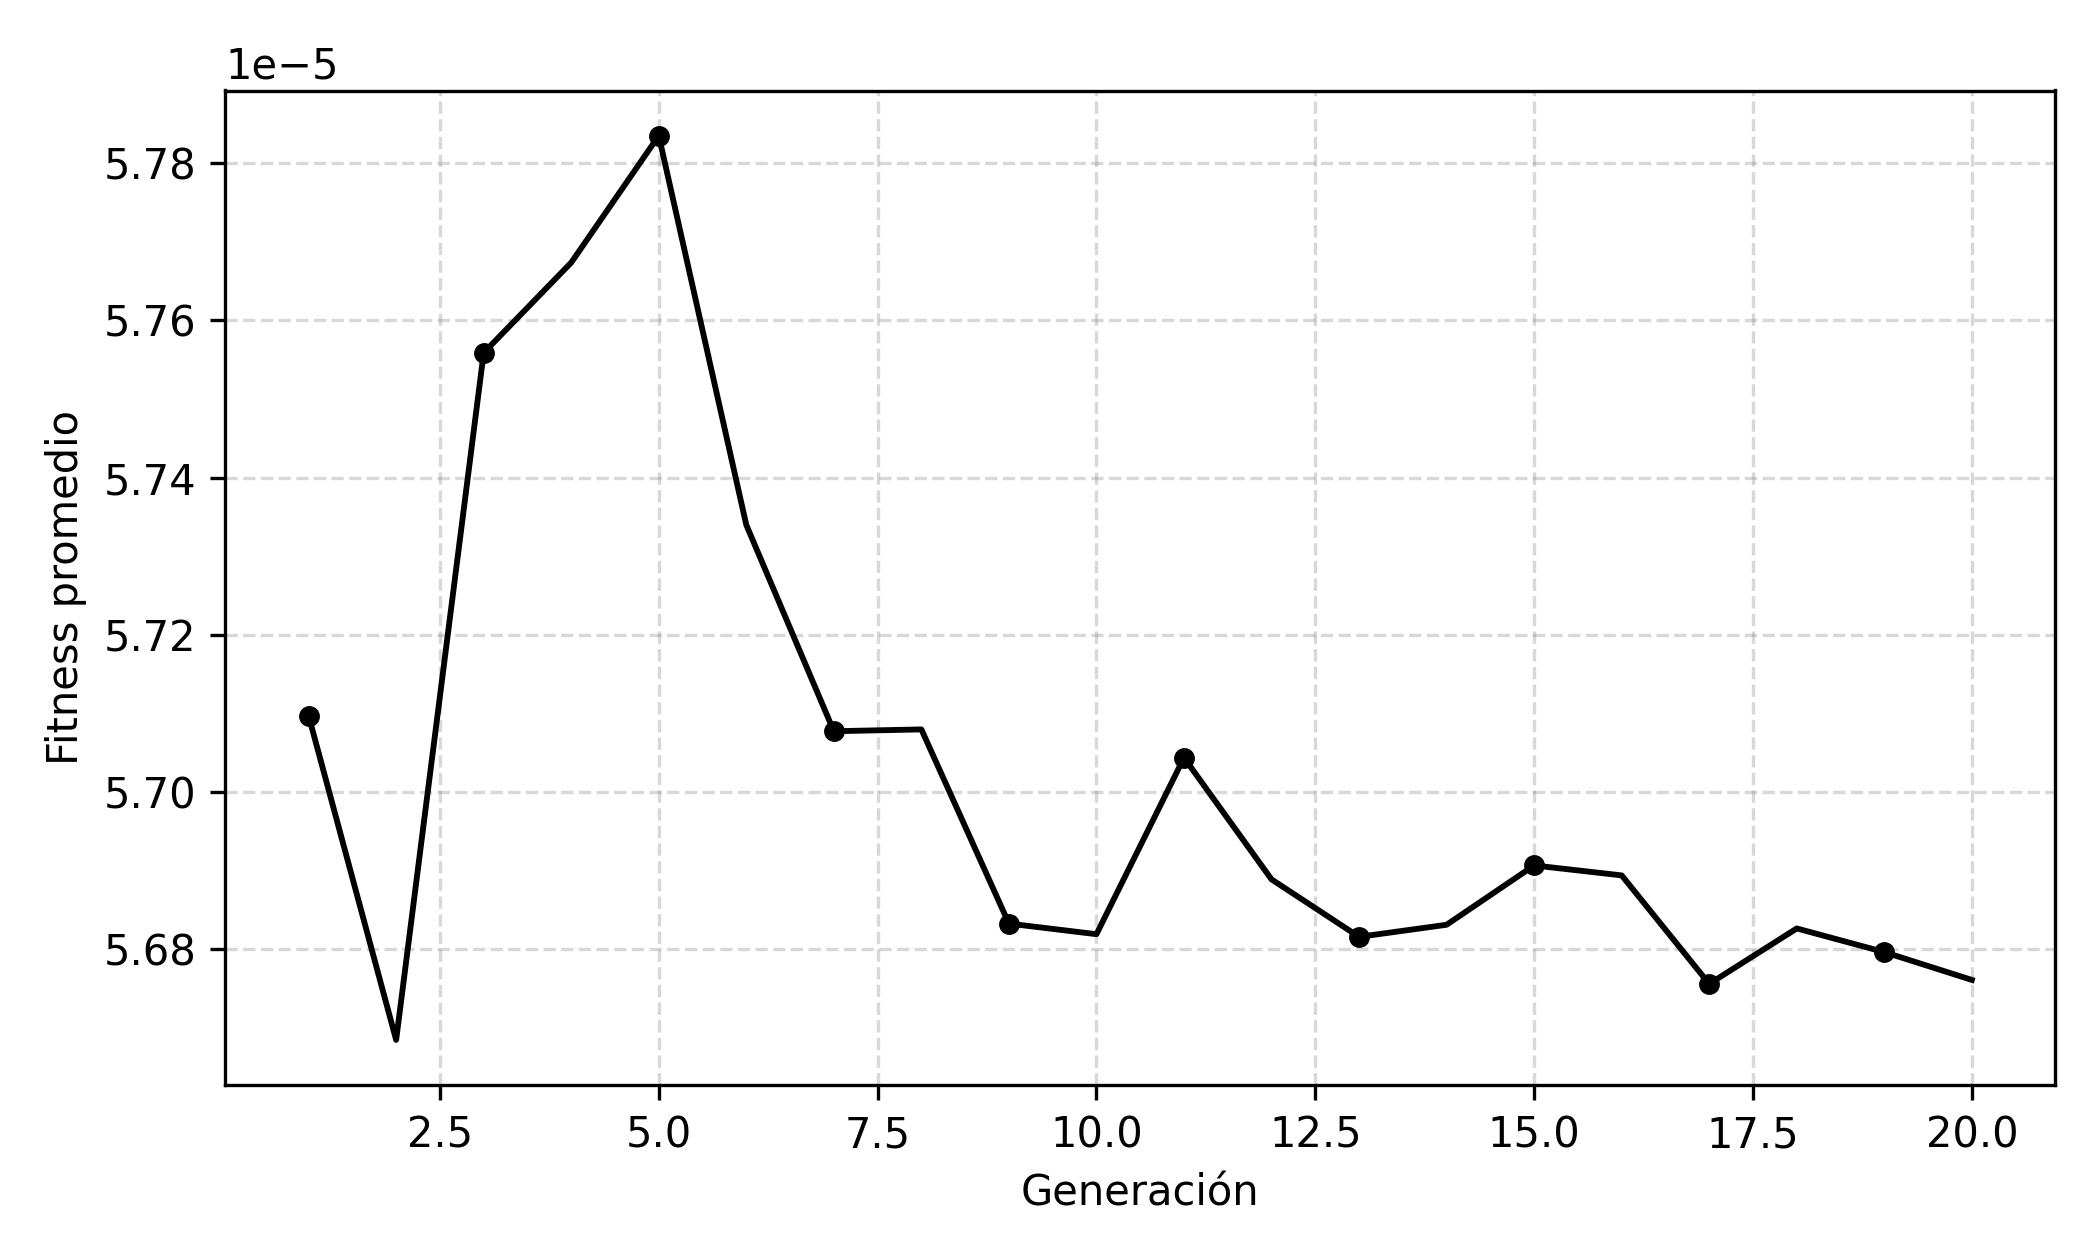
\includegraphics[width=\linewidth]{assets/figures/fitness_promedio_bn.png}
\end{center}
\artFiguraCaption{Fitness promedio por generación, sobre la muestra real de CICIDS2017.\label{fig:convergencia}}

Como se observa en la Figura~\ref{fig:convergencia}, el fitness promedio de la población mejora de forma irregular a lo largo de las 20 generaciones, con retrocesos puntuales: es el comportamiento esperable de la selección por ruleta, cuya presión selectiva es proporcional al fitness y no garantiza por sí sola una mejora monótona del promedio poblacional, aunque el mejor individuo global nunca se pierde. La tabulación completa por generación y la distribución final de carga se documentan en la carpeta \texttt{outputs/} del repositorio.

% ---------------------------------------------------------
% Discusión
% ---------------------------------------------------------
\artSection{Discusión}

La selección por ruleta asigna a cada individuo una probabilidad de reproducción proporcional a su fitness, lo que la vuelve sensible a la escala y a la dispersión de los valores de aptitud de la población: cuando los fitness son muy parecidos entre sí, la presión selectiva se diluye y la búsqueda pierde capacidad de discriminar entre buenas y malas soluciones. Esto explica la evolución irregular observada en la Figura~\ref{fig:convergencia}, con generaciones donde el fitness promedio retrocede antes de volver a mejorar; el mejor individuo global, sin embargo, se conserva siempre porque se registra de forma independiente de la población corriente en cada generación.

Este resultado se relaciona con la literatura revisada: el backlog observado (386 de 500 alertas) es una manifestación cuantitativa del \textit{alert overload} descripto por Jalalvand et al. \cite{ref1}, y el desbalance de carga entre analistas es el tipo de causa estructural de \textit{alert fatigue} señalada por Tariq et al. \cite{ref2}: un modelo de asignación que ignore la carga acumulada tiende a perpetuar ambos problemas. A diferencia de los enfoques de priorización adaptativa basados en aprendizaje automático \cite{ref3}, que requieren datos históricos etiquetados y reentrenamiento periódico, el enfoque evolutivo aquí propuesto no necesita entrenamiento previo, en la misma línea que los antecedentes de algoritmos genéticos aplicados a \textit{Job Shop Scheduling} \cite{ref4} y a balanceo de carga en sistemas distribuidos \cite{ref5}. Como posible aplicación, el mismo esquema de representación cromosómica y operadores canónicos resultó igualmente aplicable al pasar de un dominio sintético a tráfico real de un ataque DDoS, lo que sugiere que es extensible a otras fuentes de alertas (por ejemplo, eventos de un SIEM en producción) sin cambios estructurales.

% ---------------------------------------------------------
% Conclusiones
% ---------------------------------------------------------
\artSection{Conclusiones}

El modelo propuesto pone a prueba la hipótesis de que la asignación de alertas de un SOC puede formularse y resolverse como un problema de optimización combinatoria mediante un Algoritmo Genético Canónico, obteniendo una asignación medible y verificable. Los resultados sobre datos reales de CICIDS2017 confirman esa hipótesis: el algoritmo produjo una asignación válida, con fitness, tiempo total y desbalance de carga cuantificados generación a generación.

Cada uno de los objetivos específicos --representación cromosómica, función de fitness, implementación del operador de selección por ruleta, registro de la evolución del fitness, cuantificación de la distribución final de carga y medición del tiempo de ejecución-- quedó verificado sobre datos reales. Algunos aspectos quedan abiertos para continuar la investigación con el software desarrollado como base: comparar el resultado obtenido contra una asignación manual o basada en reglas fijas como línea de base explícita, evaluar el modelo sobre alertas provenientes de un SIEM en producción, y ajustar el tamaño de población y el número de generaciones para estudiar el compromiso entre calidad de la solución y costo computacional.

% ---------------------------------------------------------
% Referencias
% ---------------------------------------------------------
\begin{thebibliography}{99}
\setlength{\itemsep}{0.4em}
\small

\bibitem{ref1} Jalalvand, F.; Baruwal Chhetri, M.; Nepal, S.; Paris, C. (2025). «Alert Prioritisation in Security Operations Centres: A Systematic Survey on Criteria and Methods». \textit{ACM Computing Surveys}, 57(2). \url{https://dl.acm.org/doi/10.1145/3695462}

\bibitem{ref2} Tariq, S.; Baruwal Chhetri, M.; Nepal, S.; Paris, C. (2025). «Alert Fatigue in Security Operations Centres: Research Challenges and Opportunities». \textit{ACM Computing Surveys}, 57(9), art.\ 224. \url{https://dl.acm.org/doi/10.1145/3723158}

\bibitem{ref3} «Adaptive Alert Prioritisation in Security Operations Centres via Learning to Defer with Human Feedback» (2025). arXiv:2506.18462. \url{https://arxiv.org/abs/2506.18462}

\bibitem{ref4} «Algoritmo Genético Simple para Resolver el Problema de Programación de la Tienda de Trabajo (Job Shop Scheduling)» (2018). SciELO Chile. \url{https://www.scielo.cl/scielo.php?script=sci_arttext&pid=S0718-07642018000500299}

\bibitem{ref5} Luna Rosas, F. J.; Tristán Ávila, R.; Martínez Pedroza, J. de J. (2003). «Aplicando un algoritmo genético para balancear carga dinámicamente en ambientes distribuidos orientados a objetos (CORBA)». \textit{ConCiencia Tecnológica}, N.\textdegree{} 23. \url{https://dialnet.unirioja.es/servlet/articulo?codigo=6482681}

\bibitem{ref6} Sharafaldin, I.; Lashkari, A. H.; Ghorbani, A. A. (2018). «Toward Generating a New Intrusion Detection Dataset and Intrusion Traffic Characterization». \textit{Proceedings of the 4th International Conference on Information Systems Security and Privacy (ICISSP)}, pp.\ 108--116. \url{https://www.unb.ca/cic/datasets/ids-2017.html}

\end{thebibliography}

% ---------------------------------------------------------
% Datos de contacto
% ---------------------------------------------------------
\artSection{Datos de Contacto}
{\artSmall\itshape
\noindent Chacón, Agustina. Universidad Tecnológica Nacional, Facultad Regional Rosario, Zeballos 1341, S2000BQA, Rosario, Santa Fe, Argentina. aguscchacon@gmail.com\par
\vspace{0.3em}
\noindent Gomez Manna, Joaquina. Universidad Tecnológica Nacional, Facultad Regional Rosario, Zeballos 1341, S2000BQA, Rosario, Santa Fe, Argentina. gomezmannajoaquina@gmail.com\par
\vspace{0.3em}
\noindent Tabini, Azul. Universidad Tecnológica Nacional, Facultad Regional Rosario, Zeballos 1341, S2000BQA, Rosario, Santa Fe, Argentina. azultabini@gmail.com\par
\vspace{0.3em}
\noindent Carloni, Nahuel Iván. Universidad Tecnológica Nacional, Facultad Regional Rosario, Zeballos 1341, S2000BQA, Rosario, Santa Fe, Argentina. nahuelcarloni25@gmail.com\par
\vspace{0.3em}
\noindent Mierez, Joaquin. Universidad Tecnológica Nacional, Facultad Regional Rosario, Zeballos 1341, S2000BQA, Rosario, Santa Fe, Argentina. joakomierez1@hotmail.com\par
}

\end{document}
